
\section{Introduction}

    %%%%%%%%%%%%%%%%%%%%%%%%%%%%%%%%%%%%%%%%%%%%%%%%%%%%%
    %%%          Comments Examples:
    %%%%%%%%%%%%%%%%%%%%%%%%%%%%%%%%%%%%%%%%%%%%%%%%%%%%%
    % // ---> Inline examples (these affect the layout slightly): 
        %  \noteHidden[inline]{example of inline noteHidden}
        %  \noteInfo[inline]{example of inline noteInfo}
        %  \noteError[inline]{example of inline noteError}
        %  \noteChange[inline]{example of inline noteChange}
        %  \noteImprove[inline]{This needs noteImprove}
    
    
    %% ------------------------------------------------
    %                 Teaser Figure:
    %% ------------------------------------------------
    \begin{figure} [ht]
    
        \begin{centering}
        \begin{tabular}{c}
            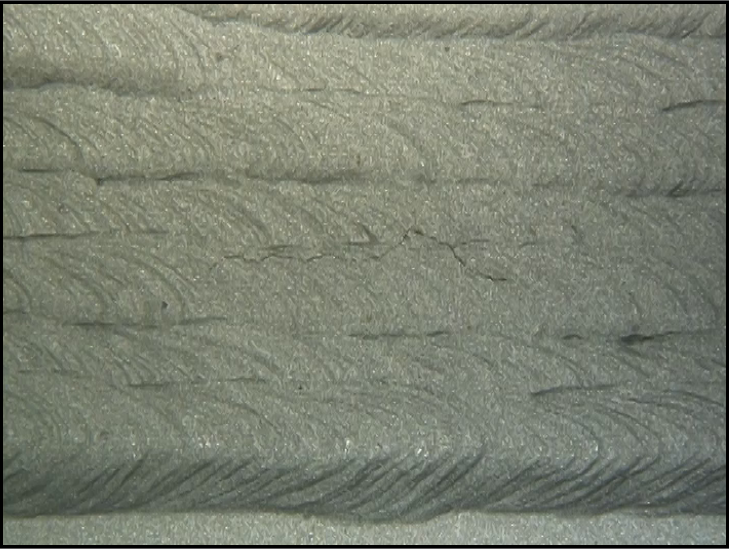
\includegraphics[width=0.8\columnwidth]{Images/WeldingCrack2.png} \\
            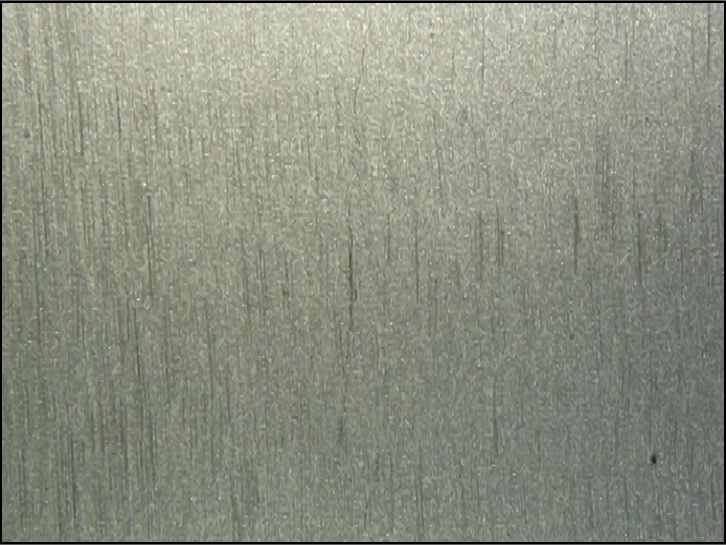
\includegraphics[width=0.8\columnwidth]{Images/ScratchCrack2.png}
        \end{tabular}
        
        \caption{A few examples of the challenges in detecting cracks in power plants such as: substantial texture due to welding (top), grind and scratch marks (bottom). Though hardly visible due to low contrast and surrounding textures, each of the two images contain only a single crack which we have conveniently centered in the image.}
        \label{challenges}
        \end{centering} 
    \end{figure}
    %% ------------------------------------------------
    
    Structural components of nuclear power plants require periodic inspection to ensure safety requirements and uninterrupted services. The inspection helps agencies to predict future conditions, support investment planning, and allocate limited maintenance and repair resources \cite{Koch:2015}. Typically, certified inspectors or structural engineers manually monitor the videos recorded along the concrete surfaces of the power plant and detect any development of cracks or crack-like defects. Since cracks are rare occurrences, manual inspection is a labor-intensive and tedious process of evaluating 100+ hours of video. Furthermore, since it is costly to close down the power plant for closer investigation, concerns raised by a human inspector about elevated development of cracks needs to be identified and validated for false alarms. Utilization of computer vision for automated crack detection to be used side-by-side with the inspectors is of great interest, not only to reduce false alarm rates and alleviate effort of the inspectors, but also aid in catching more crack related defects onsite. \noteHidden{@Min, would the following sentence describing a crack detection task fit?} Given an input video, the task of an automated crack detection method is to identify a set of frames in that video that contain one or more cracks.
    

  Automatic crack detection poses several challenges, of which a few are depicted in figure \ref{challenges}. First, although the cracks may be modeled as thin edge-like segments, a general model to discriminate a wide range of appearances is very difficult due to lighting and shading conditions at different locations. Second, the images in the recorded video contain highly textured areas including weld and concrete surface which causes fragmented and noisy segmentations. Third, the background from cracks often involves differentiating noise such as scatches and grind patterns which can has similar appearences to cracks. The distinction among scatches, grinds, and cracks becomes even more difficult when an actual crack either overlapped with a scatch or appear inside a grind area.
    

    Summary of recent crack detection methods in the domains of reinforced concrete bridges, precast concrete tunnels, underground concrete pipes, and asphalt pavements can be found in \cite{Koch:2015}.  Most methods follow two steps:
    (1) detection of local features, often using textures; 
    (2) classification of (grouped) features.
    
    Local features have been detected using morphological operations \cite{jahanshahi2013}, Gabor \cite{Medina2014}, 
    \comment{list out what types of texture features} texture features and SVM \cite{chanda2014}, HOG \cite{Kapela2015}, 
    
    
    \comment{List out the features that previous methods have used.  Then briefly mention how many of these are based on a small window.}  The noisy/missing features are filtered/connected using
    segment extending \cite{Liu2008}, tensor voting \cite{Zou2012}, extending a saliency map \cite{Xu2013}, seed growing \cite{Li2011}. 
    
    Then, grouped features have been classified using geometric features with neural network \cite{jahanshahi2013}, 
    
    
    \comment{DON't KNOW WHERE THE REST  FITS in}
    A block SVM classifier with Hough features was used to detect cracks in noisy images HTF-SVM \cite{Hu2010}. 
    
    Unsupervised learning method have also been applied to detect road cracks \cite{Oliveira2014}. 
    
    
    Gabor features along with an Adaboost classifier are used to detect road cracks . Chanda et. al  detect cracks in highly textured bridges using . Kapela et. al. detect asphalt using HOG and a SVM classifier \cite{Kapela2015}. Prasanna et. al. divide the image into blocks, detect lines using RANSAC in each block, extract gradient and intensity features from the block at different scales and then classify the block as crack or not using a classifier \cite{Prasanna2014}. 
    
    
    
    \comment{NOT SURE WHERE THIS FIT IN: and crack saliency \cite{Xu2013}} 
    
    
    
    
    \comment{List them here}.  All methods uses input of single frame thus do not use the spatial-temporal aspects of features.   
    % (I can't think of how to relate Zou) Zou et. has recently used Kalman filter detect defects in weld pipe inspection videos by using a Kalman filter to detect the continuity of the defect motion as compared to just noise detections \cite{Zou2015}. 
    
    
    We propose to improve detection accuracy in two ways.  First, we improve the accuracy of local patches detection by learning features with convolutional neural network.  We collected \comment{XXX} labeled local patches to fine-tune the deep network.  Second, we leverage the expection motion pattern of camera during imaging to group detected local patches in spatio-temporal space, then classify at a group level.  Evaluation using 17 real videos with nearly \comment{170,000 frames of video} demonstrate that spatial-temporal grouping provides \comment{XXX}\% improvement in F-score achieving 86\% true positive rate and 4\% false positive rate.  When compared against two recent methods, our method performed 0.40 higher in F-score on our crack dataset.  
     
     

    % In a survey paper by Koch et. al \cite{Koch:2015} different methods for detecting defects civil infrastructures  were discussed extensively. The authors summarize the different methods of crack detection in the domains of reinforced concrete bridges, precast concrete tunnels, underground concrete pipes, and asphalt pavements. They generalize that all the methods usually have two steps, pre-processing, and crack-identification. The pre-processing involves extracting features from lines or edges. They categorize crack-identification step into 3 categories, threshold-based, model-based, and pattern-based approaches. 

    %% ------------------------------------------------
    %                 Overview Figure:
    %% ------------------------------------------------
    \begin{figure*}
    
        \begin{centering}
        
            \includegraphics[width=0.6\textwidth]{Images/CrackDiagramDraft.png}
        
            \caption{(Obviously an idea draft) This figure represents the method at an abstract level in a brief glance.}
            \label{fig:FigMain}
            
        \end{centering}
        
    \end{figure*}
    %% ------------------------------------------------

    \paragraph{Related Works}
        Much of the previous research in automatic crack detection has focused on developing a trained classifier using some hand-crafted features. For instance, 
        
        
        
        To reduce false positives, statistical features such as seed growing \cite{Li2011} and crack saliency \cite{Xu2013} have also been applied. 
        
        
        Jahanshahi et al. segment line-like segments using morphological operations, extract geometric features from the segments and then use a neural network classifier to determine if the segment is a crack \cite{jahanshahi2013}. A block SVM classifier with Hough features was used to detect cracks in noisy images HTF-SVM \cite{Hu2010}. Oliveira et. al develop a system to detect road cracks using an unsupervised learning method \cite{Oliveira2014}. Gabor features along with an Adaboost classifier are used to detect road cracks \cite{Medina2014}. Chanda et. al  detect cracks in highly textured bridges using texture features and SVM \cite{chanda2014}. Kapela et. al. detect asphalt using HOG and a SVM classifier \cite{Kapela2015}. Prasanna et. al. divide the image into blocks, detect lines using RANSAC in each block, extract gradient and intensity features from the block at different scales and then classify the block as crack or not using a classifier \cite{Prasanna2014}. Zou et. al detect defects in weld pipe inspection videos by using a Kalman filter to detect the continuity of the defect motion as compared to just noise detections \cite{Zou2015}. 
    
        Instead of hand-crafting the features, Convolutional Neural Networks (CNN) have been utlized to learn features that are useful to the classification task. Use of CNN has met great success in object classification in recent years with the monumental success of Alexnet in the 2012 ImageNet competition \comment{\cite{krizhevsky2012imagenet}}. The GoogLeNet CNN, which is modeled to have less parameters but deeper, performed the best in the 2014 ImageNet Competition \comment{\cite{googlenet2014going}}. Deep Learning CNNs learned in the multi-class object classification can be fine tuned to other tasks such as face detection \comment{\cite{farfade2015multi}} and style classification \comment{\cite{karayev2013styleRecognizing}}. 
        % However, the GoogLeNet framework is too generalized in the context of crack detection \comment{@Steve, can you confirm this?} and its parameters are still in need of fine-tuning to achieve desirable detection performance with a wide range of background pattern and texture.


        Both illumination and contrast vary as a camera is moved across a power plant wall during inspection. If solely classified on individual image patches within the frames then textures such as scratches, welding and grind marks can be frequently and incorrectly considered cracks if the classifier is not strick enough.
        % As previously stated, these false positive detections can be problematic and costly.
        Simply modeling the crack classifier on image patches to be more conservative to reduce false alarms risks reducing its ability to successfully classify actual cracks. 
        Since the inspection for cracks is captured in a sequence of images, we propose to leverage camera motion in video to add spatio-temporal constraint to group and classify detected crack patches. 
        In this paper, we propose to improve the detection of cracks by (1) fine-tuning the GoogLeNet convolutional neural network for crack block classification, and (2) group the detected crack patches by fitting planes in the spatial-temporal space.
        Testing on 17 real videos demonstrates accuracy of \comment{[XX] TP} and \comment{[XX] FP} rates which is \comment{[XX]\%} improvement over prior method. Testing of 42 real images demonstrates 38\% improvement over prior method. %Note that the evaluation of the method is conducted at the classification of image level rather than the segmentation at pixel-level.